\documentclass{article}
\usepackage{hyperref}
\usepackage{ulem}
\usepackage{amssymb}
\usepackage{parskip}
\usepackage{graphicx}
\graphicspath{ {./} }
% pandoc Rules.tex -f latex -t html5 -o Rules.htm --pdf-engine=lualatex --css=..\page\style.css --self-contained

\title{Plane Builder Rules}

\begin{document}

These are the rules you'll use to create airplanes. This is an involved
and complex project, but you can do it!

\section{Plane Building Stats}
\label{_Plane Building Stats}

Here's a list of the Stats that matter for airplanes as you build.

Input Stats

\begin{itemize}
    \item          Mass: Mass is how much stuff weighs. Keeping your mass low is a
          priority, but engines get a lot bigger as they get more powerful, so
          it matters less and less over time.
    \item          Drag: Drag is how much stuff catches airflow, slowing the plane
          down. Lower is better.
    \item          Structure: Used to determine how tough an airplane is overall.
          Structure is used as a cap for Maximum Strain and will eventually
          relate to the Toughness stat. Higher is better.
    \item          Stability: Used to determine how stable the aircraft is in
          flight. It is divided into two stats, which will be synthesized at the
          end to create the final Stability stat. Less or more is dependent on
          what you want the aircraft to do.

          \begin{itemize}
              \item                    Lateral Stability: Combines Yaw and Roll stability. Usually
                    lower, especially on planes with high torque.
              \item                    Pitch Stability: Usually the higher of the two, this stat is
                    more easily changed.
          \end{itemize}
\end{itemize}

\begin{itemize}
    \item          Control: How much control the aircraft has. More is better.
    \item          Cost: How much money everything costs. More costs more.
    \item          Sections: How physically large the aircraft's hull is. More
          means a larger, heavier aircraft.
    \item          Wing Area: How large a wing is. Larger induces more drag but
          also lifts heavier planes.
    \item          Wing Span: How long a wing is. Longer is more efficient for
          drag and more stable, but more fragile and lowers Control.
    \item          Lift Bleed: How efficient the wings are. Lower is better.
    \item          Power: How much go the engine has.
\end{itemize}

Output Stats

\begin{itemize}
    \item          Top Speed: How fast the plane flies.
    \item          Boost: How fast the plane accelerates.
    \item          Dropoff: The point of speed at which your engine is more or
          less efficient.
    \item          Stall Speed: How slow the plane can go before it falls out of
          the sky.
    \item          Handling: How well the aircraft handles.
    \item          Structural Integrity: How tough the plane is. Basically HP.
          Divided into two stats.
    \item          Maximum Strain: How much G-Forces the plane can take.
    \item          Toughness: Excess health.
    \item          Visibility: How hard it is to see out of the plane.
    \item          Stability: How well the plane doesn't accidently flip over.
    \item          Fuel Capacity: How much fuel the plane carries.
    \item          Stress per Flight: How hard the plane is to fly for a while.
\end{itemize}

Safety Stats

\begin{itemize}
    \item          Crash Safety: How safe it is to crash land.
    \item          Escape: How easy it is to get out in a hurry.
    \item          Upkeep: How much the aircraft costs per routine (standard game
          only).
\end{itemize}

\subsection{Basics}
\label{_Basics}

Planes are built out of components. We're going to build it one part at
a time in the following order.

\begin{itemize}
    \item  \hyperref[_Era]{Era}: When is the plane from?
    \item  \hyperref[_Crew]{Crew}: Defining who is inside the aircraft, and passengers.
    \item  \hyperref[_Engines]{Engines}: Defining how the aircraft is powered and how it is cooled.
    \item  \hyperref[_Frame_and_Covering]{Frames and Covering}: Putting an actual frame around everything.
    \item  \hyperref[_Wings]{Wings}: Making it fly.
    \item  \hyperref[_Stabilizers]{Stabilizers}: Keeping the plane steady.
    \item  \hyperref[_Control_Surfaces]{Control Surfaces}: Steering the plane.
    \item  \hyperref[_Reinforcement]{Reinforcement}: Making sure the aircraft stays together.
    \item  \hyperref[_Weapons]{Weapons}: What the aircraft is armed with.
    \item  \hyperref[_Load]{Load}: Fuel, Bombs, and Cargo.
    \item  \hyperref[_Landing_Gear]{Landing Gear}: Where the plane meets the earth.
    \item  \hyperref[_Upgrades]{Accessories}: Upgrades to make the plane better.
    \item  \hyperref[_Propeller]{Propeller}: What type of propeller to put on the plane.
    \item  \hyperref[_Optimization]{Optimizations}: Fine-tune the aircraft.
    \item  \hyperref[_Final_Calculations]{Final Stats}: Putting it together into a profile you can use in game.
    \item  \hyperref[_Used_Planes]{Used Planes}: Rules for buying planes used.
    \item  \hyperref[_Altitude_Rules]{Altitude Effects}: What happens when you really high?
\end{itemize}

Your plane will generally need, at minimum, a pilot, an engine, and some
wings. Without wings, it's a car. Without an engine, it's a glider.
Without a pilot, it's a missile.

As you build the plane, remember planes cannot have negative Drag or
Mass; if you manage to make one like that, you will always at least have
1 MP and 1 Drag.

\subsection{Era}
\label{_Era}

Your Era will determine some factors about your aircraft to start.
Regular Flying Circus is generally WW1 Era. When you're making a real
aircraft be a little strict with the eras, a Spitfire FR.XIV is
technically from 1944 and a Last Hurrah aircraft but the engine is a WW2
one and the aerodynamics are mostly Coming Storm.

\begin{tabular}{|l|l|l|l|l|l|l|}
    \hline
    Era          & Years               & Lift Bleed & Maximum Bomb Load & Cantilever Bonus & Cost
    Adjustment   & Pitch Stability Mod                                                                 \\\hline
    Pioneer      & 1903-1914           & 30         & 1/6 Structure     & +4               & -2þ  & +0 \\\hline
    WW1          & 1915-1919           & 25         & 1/5 Structure     & +3               & 0þ   & +0 \\\hline
    Roaring 20s  & 1920-1929           & 23         & 1/4 Structure     & +1               & +5þ  & +0 \\\hline
    Coming Storm & 1930-1938           & 22         & 1/3 Structure     & 0                & +10þ & +2 \\\hline
    WW2          & 1939-1943           & 20         & 1/3 Structure     & 0                & +15þ & +2 \\\hline
    Last Hurrah  & 1944+               & 18         & 1/2 Structure     & 0                & +20þ & +2 \\\hline
\end{tabular}

Components of the aircraft are associated with an era, when they
first became widely available. For Himmilgard, this era is WWI. This is
not a hard and fast rule, airplanes commonly have features ahead of
their time, and when replicating a real airplane, simply use the
features that it actually possessed. For custom designs, it is best for
most characters to remain within the era limits with perhaps one
exception. Students, with their cutting-edge designs, may have two
components, or one component two eras ahead. As always, discuss with the
GM and the rest of the group.

\subsection{Crew}
\label{_Crew}

Each member of the crew, including the pilot, sits inside the frame of
the aircraft.

\subsubsection{Cockpits}
\label{_Cockpits}

Firstly, decide below how the cockpit is constructed by selecting one
below for each crew position.

Visibility, Flight Stress and Escape modifiers apply to each crew
position individually.

\begin{tabular}{|l|l|l|l|l|}
    \hline
    Type                                               & Description                             & Effects                    & Cost & Era \\\hline
    Open                                               & The pilot is fully exposed to the air.  & +1 Mass, +3 Drag, +2
    Escape, +1 Visibility                              & -                                       & Pioneer                                 \\\hline
    Windscreen                                         & A piece of glass in front of the pilot. & +2 Mass, +1 Drag.
    +2 Escape, +1 Visibility                           & 1þ                                      & Pioneer                                 \\\hline
    Sealed                                             & There is no window or external view.    & +2 Mass, -3 Escape, -1
    Flight Stress. This crewmember cannot see outside. & 1þ                                      & Pioneer                                 \\\hline
    Narrow Canopy                                      & A frame with small windows.             & +3 Mass, -1 Visibility. -1
    Flight Stress.                                     & 3þ                                      & WWI                                     \\\hline
    Bubble Canopy                                      & A cockpit made from curved glass.       & +3 Mass, -3 Drag, -1
    Flight Stress                                      & 8þ                                      & WWII                                    \\\hline
\end{tabular}

To each cockpit, you can add the following upgrades.

\begin{tabular}{|l|l|l|l|}
    \hline
    Upgrade                                          & Description                                                 & Cost    & Era         \\\hline
    Co-Pilot Controls                                & Allows this seat to also control the aircraft. -2
    Flight Stress for Pilots.                        & 1þ                                                          & Pioneer               \\\hline
    Escape Hatch                                     & +1 Mass, +3 Escape                                          & 2þ      & Pioneer     \\\hline
    Ejection Seat                                    & +2 Mass, +5 Escape                                          & 4þ      & Last Hurrah \\\hline
    Connectivity                                     & Connects this cockpit to any other cockpit with the same
    upgrade. +1 Mass.                                & -                                                           & Pioneer               \\\hline
    Oxygen Mask                                      & The pilot ignores the effects of high altitude and negates
    up to 2 G-Penalty. Requires 1 Charge Continuous. & 2þ                                                          & WWI                   \\\hline
    Isolated                                         & A basket or box allowing unusual mounts (like in front of a
    propeller) completely ignoring the usual system. +5 Drag, +1 Mass, +2
    Visibility, -2 Escape, +1 Flight Stress.

    Take double Injury when you Go Down.             & 1þ                                                          & Pioneer               \\\hline
\end{tabular}

These cockpit options can represent different ideas depending on
the crew area. The Narrow Canopy represents the glass panels of the
B-17's cockpit and Open the hole cut out in the wall for the waist
gunner, for example.

\subsubsection{Safety}
\label{_Safety}

Try not to die! You need to buy these upgrades on a per-cockpit basis.

\begin{tabular}{|l|l|l|l|}
    \hline
    Type                 & Effects                                                        & Cost        & Era          \\\hline
    Padding              & Negate 1 Injury for this position when you Go Down.            & 1þ          &
    Pioneer                                                                                                            \\\hline
    Harness              & Negate 1 Injury for this position when you Go Down, -1 Escape.
                         & 1þ                                                             & Pioneer                    \\\hline
    Fast Release System  & +2 to Escape.                                                  & 1þ          & Coming Storm \\\hline
    Roll Bar             & +2 Mass. Negate 1 Injury for this position when you Go Down.
                         & -                                                              & WWI                        \\\hline
    Flare Slot           & Allows flares to be fired out of a closed cockpit without
    opening the cockpit. & 1þ                                                             & Roaring 20s                \\\hline
    Basic Fan            & Requires the Electrics Vital Part.                             & -           & Pioneer      \\\hline
\end{tabular}

\subsubsection{Gunsights}
\label{_Gunsights}

These can help you aim! By default, we assume a plane has little more
than some simple ring sights. These gunsights can help you do better.
You can only use one at a time, though.

Each gunsight you stuff in your cockpit gives -1 Visibility, so
be sparing!

\begin{tabular}{|l|l|l|l|}
    \hline
    Type                                                  & Effects                                        & Cost & Era \\\hline
    X1 Collimated Gunsight                                & +1 to Attack.                                  & 2þ   & WWI \\\hline
    Telescopic Gunsight                                   & +2 to Attack if you Draw a Bead.               & 3þ   & WWI \\\hline
    Illuminated Reflex Sight                              & +2 to Attack. Disabled when the Electrics
    Vital Part is hit.                                    & 6þ                                             & WWI        \\\hline
    Gyro Gunsight                                         & {+2 to Attack, and additional +2 if you Draw a
    Bead. Disabled when the Electrics Vital Part is hit.} & {12þ}                                          &
    {WWII}                                                                                                              \\\hline
\end{tabular}

\subsubsection{Bombsights}
\label{_Bombsights}

Bombsights help put bombs on target!

A bombsight costs 2 thaler for a basic Quality 4 model, and then
+1 thaler for every 3 Quality after that.

\subsubsection{Passenger Capacity}
\label{_Passenger_Capacity}

Capacity for 5 passengers takes up 2 hull sections that cannot be used
for anything else. In-flight snacks must be purchased separately. The
passenger area is treated collectively as a crew position, so can be
connected to the crew positions with a Connectivity upgrade.

A bed, stretcher, or first-class accommodations take up 2
passenger seats.

Every Passenger on an aircraft (a person on or in the plane who
does not operate one of its functions) adds 1 Bomb Mass. As with other
forms of load, we round this up to the nearest MP.

Passenger space can be used as cargo, with every passenger seat
or stretcher being used to hold 1 Cargo. This is to represent the space
restrictions caused by seats etc.

\subsection{Engines}
\label{_Engines}

Engines come in two general types, Pusher engines and Tractor engines.
Tractor engines have the propeller ahead of the plane pulling it, while
pushers have it behind the plane pushing it away.

\subsubsection{Choosing your Engine}
\label{_Choosing your Engine}

Your engine can be chosen from the list of premade engines appropriate
to the setting, or made in the engine builder otherwise.

Generally speaking, air cooled engines are lighter but less powerful
while water cooled engines are heavier but more powerful.

\subsubsection{Mounting your Engine}
\label{_Mounting your Engine}

Engines can be mounted in a variety of ways.

A rear-mounted pusher represents an engine mounted at the far end of the
aircraft's body, like the pusher engines of a Kyushu J7W. A
center-mounted pusher engine represents a pusher engine that still has a
tail, using an extended driveshaft or Farman tail to avoid imbalance.

The visibility will be the worst visibility of all the engine mounts.
Having a pusher mount doesn't help you see around a pod-mounted engine very well.

\textbf{Hull Engine Mounts}

Hull engine mounts require a Frame Slot for each engine.

\begin{tabular}{|l|l|}
    \hline
    Type                   & Description                                                   \\\hline
    Tractor                & Normal.

    Forward-firing fixed weapons will need sync gears/spinner mounts.
    Turrets cannot fire forward.                                                           \\\hline
    Center-Mounted Tractor & -2 Pitch Stability, +1 Visibility.

    Forward-firing fixed weapons will need Sync gears. Will require an
    Extended Driveshaft.

    With the space free at the front of the aircraft, you can mount a single
    weapon that fires through the spinner.

    (Represents P-39 style engine mounts.)                                                 \\\hline
    Rear-Mounted

    Pusher                 & -4 Pitch Stability, +2 Visibility, -2 Escape.

    Rearward-firing fixed weapons will need sync gears/spinner mounts.
    Turrets cannot fire backward.

    (represents engines mounted at the rear of the aircraft)                               \\\hline
    Center-Mounted Pusher  & -2 Pitch Stability. +2 Visibility, -2 Escape.

    Requires Extended Driveshaft, Farman Tail, Swept Wings w/ Rudders, or
    Boom Tail.

    Rearward-firing fixed weapons will need sync gears/spinner mounts.
    Turrets cannot fire backward.

    (represents engines mounted in the center of the aircraft a la the
    DH2)                                                                                   \\\hline
    Pod                    & +5 Drag and -2 Visibility. Keeps the engine out of the way of
    everything.                                                                            \\\hline
\end{tabular}

\textbf{Wing Engine Mounts}

\begin{tabular}{|l|l|}
    \hline
    Type             & Description                                            \\\hline
    Nacelle (Inside) & Reduces Max Strain by half the mass of the engine. +1
    Lift Bleed.                                                               \\\hline
    Nacelle (Offset) & Adds Drag equal to the mass of the Engine.             \\\hline
    Channel Tractor  & -1 Lift Bleed. Reduces Max Strain equal to the mass of
    the engine.                                                               \\\hline
\end{tabular}

If you wanted to, you could build a plane asymmetrical, with
different engine types on either side of a wing, or a single large
engine on one wing. In these cases, take -3 Lateral Stability.

\subsubsection{Engine Torque and Rotaries}
\label{_Engine Torque and Rotaries}

Engines have Torque, which is subtracted from their Lateral Stability
directly if it uses any hull mounts. Wing and Pod mounts minimize the
stability effect of Torque, so ignore it there.

Rotary engines are usually the only engines that you need to worry about
this with in early aircraft, seeing as they are a giant chunk of metal
spinning at high speeds.

Wing mounted rotary engines reduce your Strain by the Torque (use all
engines), representing the force against the wing. In a push-pull
configuration, you can choose to reduce Structure instead.

Fuselage Push-Pull engines can also choose to reduce Structure, in which
case this negates the stability effect of Torque, and removes the rotary
bonus to dogfighting.

Contrarotary engines are a special engine type that halve the Torque
from the engine. They must be paired with a Geared Propeller in order to
function.

\subsubsection{Push-Pull Configuration}
\label{_Push-Pull Configuration}

A Push-Pull configuration allows two engines to be mounted along the
same line. This requires the same engine model be used for both.

In any Push-Pull configuration, use only the Drag from one engine, and
apply the following modifiers.

\textbf{Push-Pull Designs}

\begin{tabular}{|l|l|}
    \hline
    Type                      & Description                                             \\\hline
    Tractor + Pusher/Rearward & 90\% Engine Power. The -2 Pitch Stability
    and -2 Escape from having a Pusher. Cowling costs +2 for the Pusher
    engine as normal.                                                                   \\\hline
    Nacelle/Nacelle           & 80\% Engine Power. Only apply the nacelle penalty for
    one engine.                                                                         \\\hline
    Tandem Pod                & 90\% Engine Power. Only apply the +5 Drag Penalty once. \\\hline
\end{tabular}

\subsection{Engine Upgrades}
\label{_Engine_Upgrades}

\subsubsection{Extended Driveshafts}
\label{_Extended Driveshafts}

An extended driveshaft basically means that, while the engine is mounted
in the middle of the plane, the propeller can still be at either end
because the rod connecting the two is longer than usual and runs through
the length of the plane.

Extended driveshafts add +1 Mass.

This can be done for a variety of reasons. On tractor planes, this can
allow an artillery weapon to be mounted internally, firing through the
propeller without the use of the sync gear by running the barrel
directly through the prop hub. For example, a weapon mounted ahead of
the engine in a dedicated space like the 37mm autocannon in the nose of
the P-39 Airacobra.

On a central engine mount pusher plane, an extended driveshaft
eliminates the need for a Farman tail. You can just mount a conventional
tail around the engine without any problems. Similarly, a center-mounted
tractor with canards (ie: the tail is in front of the plane) may use the
extended driveshaft to avoid the Farman tail.

\subsubsection{Outboard Propellers}
\label{_Outboard Propellers}

Outboard Propellers are when a set of belts, gears, and pulleys are used
to offset the propeller (or propellers) to the side of the engine and
the fuselage. This requires the extended driveshaft upgrade, and incurs
a cost of +3 Drag and -2 Reliability. As a benefit, fuselage mounted
guns no longer need to be synchronized, because the propellers are out
of the way.

This upgrade can be applied to Tractor, Center-Mounted Tractors, and
Push-Pull Engines. In the case of Push-Pull engine, it is the rear
engine that drives the outboard propellers, and as such forward firing
guns still need to be synchronized, but there is no -2 penalty to
Escape.

\subsubsection{Geared Propeller}
\label{_Geared Propeller}

This upgrade can be applied to any engine. It costs +1þ for each
iteration. Available in the WWI era.

Adding this will add +50\% to the engine's Overspeed, and give -1
Reliability. You can add this as many times as you want.

You can pay an additional 1þ to negate Reliability penalty from the
geared prop only, 1-1. Available in the Roaring 20s era.

\textbf{Note:} While technically you can gear a Rotary engine (and
there are a few historical examples), this is an abomination against
engineering and you should think twice, or a dozen times before doing it.

\subsubsection{Cowling}
\label{_Cowling}

Cowling can be applied to any air-cooled engine.

\begin{tabular}{|l|l|l|l|l|}
    \hline
    Type                 & Description                                      & Engine Types & Cost    & Era     \\\hline
    Basic Cowl           & 80\% Engine Drag, +1 Mass.                       & Air Cooled   & 1þ      & Pioneer \\\hline
    Rotary Basic Cowl    & 40\% Engine Drag. +1 Mass.                       & Rotary       & 1þ      &
    Pioneer                                                                                                    \\\hline
    Closed Cowl          & 30\% Engine Drag. -1 Reliability, +1 Mass.       & Rotary       & 1þ      &
    WWI                                                                                                        \\\hline
    Foil Cowl            & 40\% Engine Drag. +3 Reliability, +2 Mass.       & Air Cooled +
    Rotary               & 3þ                                               & Roaring 20s                      \\\hline
    Adjustable Slat Cowl & 50\% Engine Drag. +2 Reliability, +2 Mass.       & Air
    Cooled               & 2þ                                               & Coming Storm                     \\\hline
    Sealed Cowl          & 50\% Engine Drag. +1 Mass per 3 Engine Drag (pre
    reduction).          & Liquid Cooled                                    & 1þ           & Pioneer           \\\hline
\end{tabular}

Cowls are more difficult to apply to fuselage pusher aircraft,
requiring careful engineering for airflow. Increase the costs by +2.
The exception is Sealed Cowl, since well, they're sealed and there's no airflow
to be engineering.

Additionally, an air cooling fan can be mounted inside the
cowling of a non-rotary air-cooled engine. This can draw vast quantities
of air over the engine, though it introduces an additional heavy
spinning blade to the crankshaft.

\begin{itemize}
    \item          Air Cooling Fan: +6 Reliability, +3 Mass. Double Torque. 4þ
\end{itemize}

\subsubsection{Turbocharger}
\label{_Turbocharger}

A turbocharger takes up a frame slot!

\subsubsection{Engine as Generator}
\label{Engine_as_Generator}

You can mount an engine as a generator. It doesn't provide any power to
make you go forward, but you can boost it independently of your other
engines to recharge batteries or provide energy for things. You don't
require an alternator (we presume that's built in) and it generates
double Charge as the same engine if it were powering a propeller with an
alternator.

\subsubsection{Cooling (Air)}
\label{_Cooling_(Air)}

If your engine is air-cooled, awesome! Just plop that bad boy in there
and it'll go on its own. Adds the Oil Pan Vital Part.

\subsubsection{Cooling (Rotary)}
\label{_Cooling_(Rotary)}

If your engine is \emph{rotary}, you'll need to add 1 Mass for the
engine's Oil Tank. This is a separate Vital Part.

\subsubsection{Cooling (Liquid)}
\label{_Cooling_(Liquid)}

If your engine is \emph{liquid-cooled}, you'll need to add a radiator
and an oil cooler.

An oil cooler is simple: you add +1 drag per 15 power and it counts as a
Vital Part.

A radiator weighs 3 Mass and has a variable amount of Drag, which you
choose. You cannot have more radiators than you have engines, but you
can opt to connect multiple engines to the same enlarged radiator.
This'll save weight, but be a single point of failure. Each radiator is
a Vital Part.

The \emph{Drag }of a radiator is how much of the surface of the radiator
is exposed to the air. Every point of Drag gives +2 Cooling. You must
have a Cooling value equal to the Cooling of your engine(s) or lose
reliability. Every point of cooling you have less than that gives -1
Reliability. Having more Cooling than your Engine requires will not make
it more reliable.

The \emph{Type }is the design of the radiator, and the \emph{Mount} of
the radiator is where it is in relation to the engine (not the aircraft
as a whole) and it affects radiator performance after it gets shot. Both
of these can give straight reliability bonuses to the engine due to
mechanical simplicity or efficiency.

Radiators can have different types. If the radiator gains more Drag, it
will not add more Reliability: this is from the other parts of the
design like hoses or framework.

\textbf{Radiator Type}

\begin{tabular}{|l|l|l|}
    \hline
    Type                & Description       & Era          \\\hline
    Panel               & Default.          & Pioneer      \\\hline
    Box                 & +2 Drag, -1 Mass. & Pioneer      \\\hline
    Intake              & +2 Cooling +3þ.   & Roaring 20s  \\\hline
    Evaporative Cooling & See Below.        & Coming Storm \\\hline
\end{tabular}

\textbf{Radiator Mount}

\begin{tabular}{|l|l|l|}
    \hline
    Location                                       & Description                                                      & Era     \\\hline
    Low                                            & +1 Reliability. Force Cool Down when shot.                       & Pioneer \\\hline
    Inline                                         & Default.                                                         & Pioneer \\\hline
    High                                           & Bonus persists for 1 Cool Down after being shot. +1 Drag. If the
    plane is an open cockpit, will spray the pilot with the radiator fluid!
                                                   & Pioneer                                                                    \\\hline
    High Offset                                    & Requires a Parasol Wing. As per High, but -1 Lateral
    Stability, and the pilot is safe if ruptured.. & WWI                                                                        \\\hline
\end{tabular}

\textbf{Radiator Examples: }

\emph{Panel radiators are any radiator design that air
    ``passes over'', while Box radiators are
    radiators designed for air to``pass
    through''. In simplest terms, if it sticks out all ugly
    like or is in the nose, it's a box, if
    it's flat against a surface like a wing
    or the skin it's a panel.}

Intake radiators are specifically radiators built inside
specialized housings designed to funnel air and reduce drag.

\begin{itemize}
    \item          The radiator on an Albatros D.II is a High Panel radiator.
    \item          The radiator on the side of a Sopwith Dolphin or Albatros D.II
          early is a Low Box radiator.
    \item          The radiator on the nose of an SE5a or Fokker D.VII is an
          Inline Box radiator.
    \item          The radiator on a Spitfire or P-51 is a Low Intake radiator.
\end{itemize}

\textbf{Special Coolant}

Normally, a radiator is just full of water. If you want to be a fancy
engineer, you can load your radiator with special coolant as follows.
Remember to round down with cooling!

If you want to use any of the coolants marked with a *, you need to
spend +2þ to harden your radiator for it.

\subsubsection{Rare Radiator Fluid}
\label{_Rare_Radiator_Fluid}

By default, radiators are filled with~water, but if you can find
sources, you can fill~it with other fluids to increase engine
efficiency.~ You need to buy the liquid again if the radiator gets
damaged.~ If the liquid is marked with a *, you need a special hardened
radiator for them (2 thaler to upgrade).

\begin{tabular}{|l|l|l|l|}
    \hline
    Liquid       & Effects                                                      & Cost & Era         \\\hline
    Water        &                                                              & -    & Pioneer     \\\hline
    Salt Water*  & +1 Reliability (Free for Fishers)                            & 1þ   & Pioneer     \\\hline
    Mineral Oil* & Absorbs 1 Miss to Cool Down. Flammable                       & 1þ   & Pioneer     \\\hline
    Castor Oil   & As Mineral Oil, but +2 Stress if leaking                     & -    & Pioneer     \\\hline
    Glycol       & +2 Reliability                                               & 2þ   & Roaring 20s \\\hline
    Freon        & +4 Reliability. Take 1 Power Reduction while RPM is below 4. &
    3þ           & Coming Storm                                                                      \\\hline
    Ammonia      & As Freon, but causes 2 Injury when leaking                   & 2þ   & Pioneer     \\\hline
\end{tabular}
\\
\begin{tabular}{|l|}
    \hline
    Evaporative Cooling \\\hline

    An alternate way to cool a liquid cooled engine is evaporative cooling.
    This requires a sufficiently large wing (at least 5 Area per engine)
    with some sort of metal skin. Rather than running water to a radiator,
    the water is sprayed as steam into a cavity in the wings to cool it,
    where it is collected and fed back into the engine. This is more
    streamlined, but is very fragile.

    Evaporative cooling only costs the +3 Mass you'd pay to get a radiator.
    There's no Drag involved, you're just ready to go.

    The downside is that any attack with a Crit roll of 16+ will knock out
    the radiator, in addition to any other damage done or other parts
    damaged.            \\\hline
\end{tabular}

\subsubsection{Pulsejets}
\label{_Pulsejets}

Pulsejets are simply bolted somewhere onto the plane. We don't
particularly care where or in what configuration: we just know however
it was done keeps it away from any working parts.

Pulsejets cost 5þ and 1 upkeep simply for having one on your aircraft.
They're hard on airplanes.

Pulsejets produce Rumble. Rumble causes stress to crew members equal to
half the total Rumble, or 3, whichever is lower. In addition, an aircraft requires a
minimum structure of total Rumble * 10 to fly, or the vibrations shake
the aircraft apart.

\subsubsection{Jet Engines \& Rockets}
\label{_Jet_Engines_\&_Rockets}

Jet engines are mounted in one of the following ways. Jet engines carry
with them their own requirement in Frame Slots owing to their size.

\begin{tabular}{|l|l|}
    \hline
    Type                     & Description                                                   \\\hline
    Front Intake/Rear Burner & Default. Can mount up to 2 engines.                           \\\hline
    Wing Pod                 & Reduces Max Strain by half the mass of the engine. +1 Lift
    Bleed.                                                                                   \\\hline
    Pod                      & +3 Drag and -1 Visibility. Keeps the engine out of the way of
    everything.                                                                              \\\hline
\end{tabular}

\subsection{Frame and Covering}
\label{_Frame_and_Covering}

Now that you have the sections your aircraft needs, you'll need to build
them. To start, build a frame. The frame gives a basic Structure, plus
some bonuses as the plane gets bigger. Choose just one, whatever the
majority of the frame is built from, and add 1 piece per section.

Generally, we split airplanes into being made of Spars, or being made of
Ribs. If your plane is kept together by tension wires with the frame
providing compression, it's made of a Spars. If it's just a big set of
solid pieces, it's made of Ribs.

A Sopwith Camel is made of Wooden Spars. A Fokker DR.1 is made of
Steel Spars. The Junkers J.1/J4 is made of Aluminum Spars. The
Polikarpov I-16 is made of Wooden Ribs. The P-47 is made of Steel Ribs.
The P-51 is made of Aluminum Ribs.

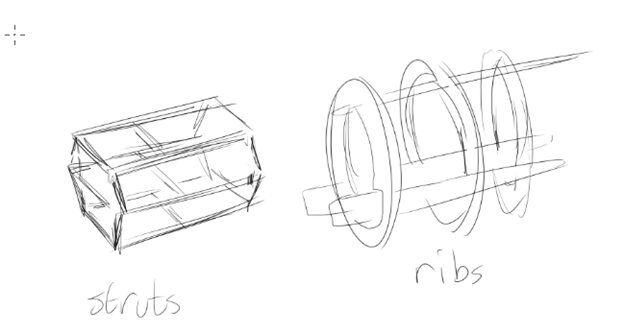
\includegraphics{Frame.png}

\begin{tabular}{|l|l|l|l|l|l|}
    \hline
    Frame Material  & Base Effect                & Cost

    Base            & Effect per Piece           & Cost

    Piece           & Era                                                                                 \\\hline
    Wooden Spars    & 15 Structure               & -          & +1 Mass, +2 Structure  & -  & Pioneer     \\\hline
    Steel Spars     & 25 Structure               & 1þ         & +1 Mass, +5 Structure  & 1þ &
    Pioneer                                                                                               \\\hline
    Aluminum Spars  & 20 Structure               & 2þ         & +½ Mass, +4 Structure  & 2þ & WWI         \\\hline
    Wooden Ribs*    & 30 Structure               & 1þ         & +2 Mass, +5 Structure  & ½þ & WWI         \\\hline
    Steel Ribs*     & 60 Structure               & 2þ         & +3 Mass, +12 Structure & 2þ & Roaring
    20s                                                                                                   \\\hline
    Aluminium Ribs* & 50 Structure               & 3þ         & +2 Mass, +8 Structure  & 3þ &
    Roaring 20s                                                                                           \\\hline
    Titanium        & -                          &            & +1 Mass, +10 Structure & 8þ & Last Hurrah \\\hline
    Living Grove*   & 30 Structure, Free Repairs & 8þ         & +2 Mass, +4 Structure
                    & -                          & Himmilgard                                             \\\hline
\end{tabular}

Titanium is a special case and cannot be used for whole frames.

A frame marked with * can be made Geodesic, which doubles the
cost per piece, but adds +50\% Structure per piece. Geodesic frame
pieces cannot subsequently be Monocoque.

By default, each frame piece adds +4 drag to the aircraft,
representing uncovered structure hanging out in the world. You must
cover these elements to make them streamlined. For each section, choose
a covering from below. The entire skin of the aircraft must be the same,
so choose the dominant type.

\begin{tabular}{|l|l|l|l|l|}
    \hline
    Skin Material                & Effects                                                 & Cost       & Monocoque

    Structure                    & Era                                                                                          \\\hline
    Naked                        & + 1 Visibility per Piece, up to +3. 60\% Airframe Mass. & -          & -
                                 & Pioneer                                                                                      \\\hline
    Cloth Canvas                 & 50\% Airframe Drag                                      & -          & -           & Pioneer \\\hline
    Transparent Celluloid        & {60\% Airframe Drag. + 1 Visibility per
    Piece, up to +3. Flammable.} & {1þ}                                                    & {-}        &
    {Pioneer}                                                                                                                   \\\hline
    Treated Paper                & 50\% Airframe Drag. Flammable. 75\% Airframe Mass       & -          &
    -                            & Pioneer                                                                                      \\\hline
    Tense Silk                   & 50\% Airframe Drag. +1 Toughness per Piece              & 1þ         & -           &
    Pioneer                                                                                                                     \\\hline
    Dragon Skin                  & 50\% Airframe Drag. Plane gains 5 Coverage AP2 armour.  &
    4þ                           & -                                                       & Himmilgard                         \\\hline
    Molded Plywood               & 40\% Airframe Drag                                      & ½þ         & +3          & Pioneer \\\hline
    Clinker Build                & 50\% Airframe Drag. Full Monocoque, adds flat +30
    Structure.                   & -                                                       & -3         & Pioneer               \\\hline
    Glass Reinforced Plastic     & 30\% Airframe Drag.                                     & 1þ         & +0          & Last
    Hurrah                                                                                                                      \\\hline
    Corrugated Duralumin         & 50\% Airframe Drag, +3 Toughness per Piece              & 1þ         &
    +10                          & WWI                                                                                          \\\hline
    Steel Sheet                  & 35\% Airframe Drag, +3 Toughness per Piece              & 1½þ        & +8          &
    Roaring 20s                                                                                                                 \\\hline
    Aluminum Sheet               & 35\% Airframe Drag, +2 Toughness per Piece. 75\%
    Airframe Mass                & 2þ                                                      & +6         & Roaring 20s           \\\hline
\end{tabular}

\subsubsection{Monocoque}
\label{_Monocoque}

You can build a monocoque (one-shell) or semi-monocoque plane if you
wish.

A monocoque or semi-monocoque plane can be built by substituting the
mass and structural bonus from a piece of frame for a
monocoque-compatible skin piece. The frame still exists: few monocoque
aircraft are truly without a frame, these frameworks are just minimized
and incorporated into the shell structure.

Monocoque skin pieces cost +1þ each, representing the labour cost of
designing and building it. This is in addition to the frame cost: that
doesn't go away.

\subsubsection{Lifting Body \& Flying Wing}
\label{_Lifting Body \& Flying Wing}

A lifting body and flying wings are both incredibly complicated
engineering achievements and require the aircraft to have a solid skin
(Molded plywood or better).

A Lifting Body aircraft counts each Frame Section (not internal
supports) as being 3m2 of wing area for the purposes of calculating
stall speed, and adds +1 Drag per piece. Each piece costs +1 thaler. For
a pure lifting body with no wings at all, Max Strain is equal to
Structure, before subtracting engine mounts, or adjusting by
optimization.

A Flying Wing is a lifting body that also avoids the extra drag
in exchange for taking +5 Lift Bleed, representing the overly thick wing
chord.

Both these aircraft still have tails, even if they are blended
into the rest of the machine.

\subsubsection{Internal Bracing}
\label{_Internal Bracing}

To increase the resilience of an aircraft, you can add Internal Bracing.
This is basically extra Frame Pieces that you don't have to put Skin on,
because it is on the inside. You can have 1 Internal Bracing piece per
actual frame section. They do not have to be the same material as
everything else: you can build a wooden aircraft with some steel
bracing, for example.

Titanium can only be used for internal bracing. Making a whole plane out
of Titanium is like making an entire ring out of diamonds: cool, but way
too expensive to be worth it.

\subsection{Tail}
\label{_Tail}

We consider the tail as the Sections of the aircraft which is left
mostly empty. They add extra frame sections, and also change the pitch
stability of the aircraft. Be very careful with your selection: a short
tail seems optimal, but pitch stability offsets the effects of things
like torque, short wings, and the natural roll instability of aircraft,
so taking it in too much will result in aircraft that are
uncontrollable.

Most of the best WW1 fighters would be Stubby, as would WW2 aircraft
like the I-16, F2A Buffalo, and Me-163 rocket fighter. As a general
rule, if you look at it and go ``that looks like a toy'', you're Stubby.
It if looks reasonable, you're Standard. Most large bombers and such
will use Long.

\begin{tabular}{|l|l|l|}
    \hline
    Location & Additional Frame Sections & Plane Modifier                                          \\\hline
    Tailless & +0                        & -4 Pitch Stability, cannot use traditional tailplane or
    vertical stabilizer. +3 Visibility                                                             \\\hline
    Stubby   & +1                        & -3 Pitch Stability.                                     \\\hline
    Standard & +2                        & No change.                                              \\\hline
    Long     & +3                        & +3 Pitch Stability.                                     \\\hline
\end{tabular}

Tail sections are as a rule empty. Tail sections aren't
necessarily at the ``back'' of an aircraft, they just bulk it out and
help balance it. For example, think of the tailgun positions in
bombers.

\subsubsection{Farman}
\label{_Farman}

If you want to mount controls behind a pusher propeller (or ahead of a
tractor!), you use a Farman Tail. This is a structure of struts built
around the propeller that allows the control surfaces to hang from it.

This is built like a regular tail, above. A farman tail weighs half as
much as a conventional Tail, but cannot be given a surface: it is always
a naked tail.

A farman tail does not count as part of a monocoque aircraft (as that
wouldn't work), so just select a type of frame material.

\subsubsection{Boom Tails}
\label{_Boom Tails}

Boom tails are another option useful for both pusher planes and some
planes with nacelles. It allows the same things as a farman tail, but is
in many ways more sophisticated. It does have some aerodynamic
difficulties, however.

A Boom Tail is built like a regular tail, and uses all the same rules.
It subtracts the Mass of the Tail from the Strain of the wings, and a
Boom Tail that isn't connected to tractor engine nacelles generates
+50\% Drag.

If you have wing warping and boom tails, you've made a mistake, and are
hit with a -2 penalty to both Lateral and Pitch Stability. A warping
wing will deflect the tailplane!

\subsection{Wings}
\label{_Wings}

You need wings to fly, or something wing-like at least. A greater wing
area means more lift on your plane, but also means more drag and less
structural integrity.

To start with, your airplane's wings have a number called their
\textbf{Lift Bleed}, determined by your Era. This represents how much
lift is lost to inefficiency in wing design. Ideally, this number would
be 1.

\subsubsection{Wing Area}
\label{_Wing_Area}

Start by deciding how much wing area you want your plane to have
overall, across all the wings. Write it down as Meters Squared.

Now, divide this area up into each wing plane your aircraft will have.
Each wing added after the first gives\ldots{}

\begin{itemize}
    \item          +3 Control
    \item          +5 Lift Bleed
    \item          -1 Visibility
\end{itemize}

\subsubsection{Aspect Ratio}
\label{_Aspect Ratio}

Wings are not all the same shape; some wings are long and skinny (they
have a \emph{high aspect ratio}) and some wings are short and wide (they
have a \emph{low aspect ratio}).

Decide the wingspan of each wing on the plane, alongside the area you've
given it.

Wings have a strain modifier and additional Drag.

Strain reduction = 2Span + Area - 10. Wings cannot generate positive
strain, how would that even work.

Wing drag is 6 * Area\^{}2 / Span\^{}2. Any given wing must always
generate at least 1 Drag.

--- The Fokker E.III has a wing area of 16 square
meters and a wingspan of 9 meters. This means the wing generates
18 Drag and inflicts a -24 Strain Penalty

--- A theoretical glider has 10 square meters of wings and a
15m wingspan. It generates just 2 drag,
but inflicts a -30 Strain Penalty.

\subsubsection{Longest Wing Effects}
\label{_Longest Wing Effects}

The longest wing on your aircraft will give the following modifier.

\begin{itemize}
    \item          8 - Wingspan = Control Modifier
    \item          Every point of Wingspan less than 8: -1 Lateral Stability.
\end{itemize}

\subsubsection{Wing Decks}
\label{_Wing Decks}

As this is a game about early flight, you may decide to have more than
one wing. Will your plane be a monoplane, a biplane, a triplane, or
something stranger?

Choose a location for each wing. Unless you are building an inline
tandem wing plane, you may have at most one Shoulder wing, one Mid wing,
and one Low wing. There's no limit on the number of Parasol or Gear
wings you can have.

The type of wing you have is determined by where it is positioned
relative to the fuselage and the centre of mass of the aircraft, which
are usually but not always in the same place.  Use the main portion of
the wing, not where it attaches.  Gull Wings may have a different attachment
point than the location of the main portion.

\begin{itemize}
    \item          A Parasol wing is on struts above the fuselage, like an
          umbrella over the aircraft.
    \item          A Shoulder wing (or High wing) is approximately at the top of the
          fuselage.
    \item          A Mid wing is around the middle of the fuselage.
    \item          A Low wing is approximately at the bottom of the fuselage.
    \item          A Gear wing is like an inverted Parasol wing, suspending the
          fuselage in the air above the wing. Gear wings can also represent
          small lift surfaces attached between the wheels of the landing gear
          using the Miniature Wing rules.
\end{itemize}

In some cases, like on the Macchi M.5 (the one Porco Rosso flew in the
war), the centre of mass might be thrown off by engine placement
significantly above or below the fuselage, so you can choose to count
wing placement relative to the engine instead.

\textbf{Wing Decks}

These apply to each full wing attached. The Largest Wing modifier
applies for Monoplanes and Sesquiplanes to the wing with the largest
Area.

\begin{tabular}{|l|l|l|}
    \hline
    Location   & Plane Modifier                                               & Largest Wing Modifier    \\\hline
    Parasol    & +3 Pitch Stability, -10 Max Strain. -2 Lift Bleed. -1
    Visibility & +1 Lateral Stability. -1 Control                                                        \\\hline
    Shoulder   & +2 Pitch Stability. -1 Lift Bleed. -1 Visibility             & -1
    Control                                                                                              \\\hline
    Mid        & -                                                            & -10\% Drag for this wing \\\hline
    Low        & -2 Pitch Stability. -1 Crash Safety. -1 Lift Bleed           & +2 Control,
    -1 Lateral Stability                                                                                 \\\hline
    Gear       & -3 Pitch Stability. -10 Max Strain, -1 Crash Safety. -2 Lift
    Bleed.     & +3 Control -1 Lateral Stability                                                         \\\hline
\end{tabular}

\subsubsection{Wing Surface}
\label{_Wing Surface}

Remember, always round down to whole numbers!

\textbf{Wing Surfaces}

\begin{tabular}{|l|l|l|l|}
    \hline
    Skin Material                      & Plane Modifier                                       & Cost/10 Area & Era                       \\\hline
    Cloth Canvas                       & -                                                    & -            & Pioneer                   \\\hline
    Treated Paper                      & Makes the plane Flammable, -1 Mass per 4 Area, up to
    25\% of the dry mass of the plane. & -                                                    & Pioneer                                  \\\hline
    Tense Silk Layers                  & 90\% Strain Penalty                                  & 2þ           & Pioneer                   \\\hline
    Plywood                            & 90\% Strain Penalty, 1 Mass/5A                       & 1þ           & Pioneer                   \\\hline
    Aluminium Sheet                    & 80\% Drag                                            & 3þ           & Roaring 20s               \\\hline
    Corrugated Duralumin               & 60\% Strain Penalty , 1 Mass/4A                      & 2þ           & WWI                       \\\hline
    Thin Sheet Steel                   & 60\% Strain Penalty, 90\% Drag, 1 Mass/5A            & 3þ           &
    Roaring 20s                                                                                                                          \\\hline
    Grand Eagle Feather                & +1 Control per 5A                                    & 6þ           & Himmilgard                \\\hline
    Solar Fiber                        & +1 Charge Gen per 5A                                 & 4þ           & Himmilgard or Last Hurrah \\\hline
    Dragon Skin                        & 40\% Strain Penalty                                  & 8þ           & Himmilgard                \\\hline
    Transparent Celluloid              & Makes the plane Flammable. +1 Visibility per
    wing. -1 Toughness per 10 Area     & 1þ                                                   & Pioneer                                  \\\hline
\end{tabular}

\subsubsection{Stagger \& Tandem Wing}
\label{_Stagger \& Tandem Wing}

If you have multiple wing decks, you may stagger the wings.

\textbf{Wing Stagger}

\begin{tabular}{|l|l|}
    \hline
    Location         & Plane Modifier                                           \\\hline
    Tandem           & Eliminates the need for Horizontal Stabilizers. +4 Pitch
    Stability. Cannot be tailless.                                              \\\hline
    Extreme Positive & +2 Pitch Stability, -2 Lift Bleed                        \\\hline
    Positive         & +1 Pitch Stability, -1 Lift Bleed                        \\\hline
    Negative         & -1 Pitch Stability, -1 Lift Bleed                        \\\hline
    Extreme Negative & -2 Pitch Stability, -2 Lift Bleed                        \\\hline
\end{tabular}

\subsubsection{Closed Wing}
\label{_Closed Wing}

Closing a pair of wings, such as by creating a box or circular
structure, eliminates the vortex effect on the end of a wing, and also
allows a more complete structure. On the other hand, this design will be
difficult to control, due to the added weight on the extreme ends of the
wings increasing the energy required to induce a roll.

Each closed wing pair costs +1 Mass, -5 Control, and +20 Max Strain.
(ie: four wings count twice, not three times)

A closed monowing isn't possible: wingtip loops to reduce drag would be
part of optimization. You can have a closed inline tandem wing though.

\subsubsection{Inline Wings}
\label{_Inline Wings}

A style of Tandem Wing where multiple wings are on the same deck level.
An inline set reduces the total drag from all wings on the same level to
75\%, but gives +3 Lift Bleed due to shadowing.

\subsubsection{Miniature Wings}
\label{_Miniature Wings}

A Wing of 2 or less square meters is a Miniature Wing. These effectively
do not count as a wing: they do not add the effects of whatever wing
deck they are added onto, and instead just add +1 Control and their size
for lift purposes. Each Miniature Wing past the first adds +1 Lift Bleed
each.

Each miniature wing must be mounted on their own deck: they can't occupy
the same space as another wing. No tandem miniature wings!

\subsubsection{Sesquiplanes}
\label{_Sesquiplanes}

If the smallest of your wings is half the size or less of your largest
wing, and the wings are not tandem, you have a Sesquiplane, an
eineinhalbdecker! This unusual configuration was used to try and get
some of the benefits of both monoplanes and biplanes. They have their
advantages, but come with structural complications.

A Sesquiplane grants

\begin{itemize}
    \item          -2 Lift Bleed
    \item          +2 Control
\end{itemize}

However, one of the following penalties will apply.

\begin{itemize}
    \item          If the smallest wingspan is less than 75\% the span of the
          largest wing, your plane generates 15\% less Tension, as you can't
          brace the wings out at the tips.
    \item          Otherwise, the plane is limited to the following external
          reinforcements: V-Struts, Single Struts, W-Struts, Wing Truss, and
          Wire Roots. It can still use any type of Cabane Strut, but the
          narrower lower wing precludes twin spar support, limiting the types of
          spars which can be used.
\end{itemize}

\subsubsection{Wing Angle}
\label{_Wing Angle}

Wings can be built at angles to change their properties. Wingtips up
(dihedral wings) improve stability, as they make the plane more likely
to roll back to a neutral position. Anhedral wings do the opposite.

Inducing a dihedral angle on the wing will add Lateral Stability, while
an anhedral wing will remove Lateral Stability instead. In either case,
your total Lift Bleed increases by the amount of stability added or
lost.

\subsubsection{Gull Wings}
\label{_Gull Wings}

Any wing can be declared a gull wing. We consider the deck of the wing
to be where the bend is, not where the root is, because this is what
matters for aerodynamic purposes. You cannot have two wings from the
same root in a non-Tandem configuration. Gull Wings are available in the
Coming Storm era.

Any Gull Wing will generate drag as though it had +10\% area, but it
comes with the following benefits:

\begin{itemize}
    \item          {A Parasol Wing can be turned into a }\emph{{Polish
                      Wing}}{. This removes the -10 Max Strain and Visibility penalty.
              Not available with Shoulder wings.}
    \item          {Mid, Low, and Gear wings can be turned into an
          }\emph{Inverted Gull Wing}{. This has the following
              effects, better for lower wings.}

          \begin{itemize}
              \item                    For Low and Mid wings, this reduces the Drag and/or Mass cost
                    of Landing Gear by 15\% (excluding Boat Hulls) and increases
                    external bomb capacity by 10\%. Not available with non-gull Mid and
                    Shoulder wings, respectively.
              \item                    For Gear wings, this reduces the Drag and/or Mass cost of
                    Landing Gear by 25\% (excluding Boat Hulls), eliminates the -10 Max
                    Strain, gives +1 Crash Safety, and increases external bomb capacity
                    by 20\%. Not available with a non-gull Low wing.
          \end{itemize}
\end{itemize}

\subsubsection{Swept Wings}
\label{_Swept Wings}

Swept Wings add +5 Lift Bleed and give -1 Lateral Stability. However,
they allow the complete elimination of the horizontal stabilizer
\emph{and} give a natural mounting point for Outboard Vertical
Stabilizers.

\subsubsection{Wingtip Weight}
\label{_Wingtip Weight}

A plane takes a -1 Control penalty for the following:

\begin{itemize}
    \item          Every 5 Mass of Weapons in Wing Mounts.
    \item          Every Wing Mounted fuel tank, internal or external.
\end{itemize}

\subsubsection{Special Wing Types}
\label{_Special Wing Types}

There are a number of special wing types. These wing types can be
combined with normal wings, but it will rarely be worth it.

\begin{itemize}
    \item          Autogyros use a rotating wing surface. They are very safe for
          light aircraft.
    \item          Helicopters power a rotating wing surface, allowing free
          vertical and horizontal movement at the cost of low stability and
          requiring a powerful engine.
    \item          Ornithopters use an engine to power a flapping effect. This
          creates supremely maneuverable but delicate and expensive craft.
\end{itemize}

Their rules will be detailed on their own pages once complete.

\subsection{Stabilizers}
\label{_Stabilizers}

An aircraft must be made stable. It must have a horizontal stabilizer to
keep the nose pointing flat, and a vertical stabilizer to prevent
spinning and rolling. You can design a plane without these things, but
it's \emph{really hard}.

\subsubsection{Stabilizer Size}
\label{_Stabilizer Size}

Airplanes need stabilizers to fly. Full stop. If you don't have them and
you haven't done something very, very clever, your plane does a wibbly
sort of motion and goes into the ground.

Your Stabilizers cost Drag, representing them getting in the airstream.

\begin{itemize}
    \item          All your vertical stabilizers will add 1/8th the total Wing
          Drag. (Minimum 1)
    \item          All your horizontal stabilizers will add 1/4th the total Wing
          Drag. (Minimum 1)
\end{itemize}

The absence of a Vertical Stabilizer subtracts Lateral Stability equal
to your Wing Area. The absence of a Horizontal Stabilizer subtracts from
Pitch Stability equal to half your Wing Area, and also adds +5 Lift
Bleed!

Tandem wing and swept wing planes don't need horizontal stabilizers:
they have enough problems. To remove them, set the selection for
horizontal stabilizers to ``The Wings''.

\subsubsection{Stabilizer Mounts}
\label{_Stabilizer Mounts}

You must choose where you mount your stabilizers. Your options
are\ldots{}

\textbf{Horizontal Stabilizer}

\begin{itemize}
    \item          Tailplane: Default
    \item          Canards (at the front): -3 Pitch Stability, Half Drag.
    \item          Outboard (on the wing): Requires either swept wings or a tandem
          wing. +1 Lateral Stability. Requires even number of stabilizers.
\end{itemize}

\textbf{Vertical Stabilizer}

\begin{itemize}
    \item          Tail fin: Default.
    \item          Outboard: Requires either swept wings, a tandem wing, or
          canards. +1 Control. Requires even number of stabilizers.
\end{itemize}

\subsubsection{Multiple Stabilizers}
\label{_Multiple Stabilizers}

You may choose to mount multiple instances of a stabilizer on your
aircraft. For example, two tail fins on your aircraft mounted on the
ends of the tailplane. As it's best when rudders and elevators are in
the airflow of an engine, you get more benefit from doing this if you
have multiple engines.

Every additional stabilizer just adds +2 drag.

For every pair of Vertical Stabilizer with an Engine beyond the first,
you get a +3 Control Bonus. If you have an extra stabilizer that isn't
paired with an engine, you get just +1 Control.

Push-pull engines count as a single engine for these purposes.

\subsubsection{V-Tails}
\label{_V-Tails}

A V-Tail combines both Pitch and Lateral Stability. It must be 1/5th the
wing drag total, gives +2 to both Stability types, and costs 5þ to
engineer. The V-Tail is from the Coming Storm era.

\subsubsection{T-Tails}
\label{_T-Tails}

A T-Tail is a horizontal stabilizer mounted at the top of (or near the
top of) the vertical stabilizer. It causes half the Drag of a
conventional horizontal stabilizer, reduces Lift Bleed by 2, and adds a
special rule to the aircraft. The T-Tail is from the WWII era.

Deep Stall: In the event of a spin/stall while above stall speed and
under power, you are at Disadvantage to recover.

\subsection{Control Surfaces}
\label{_Control_Surfaces}

Control surfaces are how an airplane moves.

You \emph{must }have some way of controlling your airplane. You need
Ailerons, Elevators and a Rudder.

\subsubsection{Ailerons}
\label{_Ailerons}

Ailerons control your airplane's rotation. You must have these!

\textbf{Ailerons}

\begin{tabular}{|l|l|l|l|}
    \hline
    Type                                             & Effects                                                & Cost    & Era     \\\hline
    No Ailerons                                      & -15 Control, -1 Crash Safety                           & -2þ     & Pioneer \\\hline
    Flap Ailerons                                    & Default                                                & -       & Pioneer \\\hline
    Wing Warping                                     & -1 Drag. Get +1 to Dogfight! at 15 speed and below.
    Reduce Max Strain equal to span of longest wing. & -                                                      & Pioneer           \\\hline
    Spoilerons                                       & When you roll Dogfight!, take +1, but then reduce your
    speed as if your Speed Factor was doubled.       & 2þ                                                     & WWII              \\\hline
\end{tabular}

Wing Warping becomes Last Hurrah era when the wing is reinforced
with cantilevers, and costs 2þ per cantilever. That's advanced
technology!

\subsubsection{Rudders}
\label{_Rudders}

Rudders give turn control and work together with ailerons and elevators
to keep the aircraft pointing in the right direction. There are two
kinds available:

\begin{tabular}{|l|l|l|l|}
    \hline
    Type          & Effects                           & Cost & Era     \\\hline
    Flap Rudder   & Default                           & -    & Pioneer \\\hline
    Flying Rudder & -1 Lateral Stability. +3 Control. & -    & Pioneer \\\hline
\end{tabular}

\subsubsection{Elevators}
\label{_Elevators}

Elevators keep your airplane's nose pointed up at the sky and not at the
ground. There are two..

\begin{tabular}{|l|l|l|l|}
    \hline
    Type            & Effects                         & Cost & Era     \\\hline
    Flap Elevator   & Default                         & -    & Pioneer \\\hline
    Flying Elevator & -1 Pitch Stability. +2 Control. & -    & Pioneer \\\hline
\end{tabular}

\subsubsection{Lift Aids}
\label{_Lift_Aids}

Flaps \& Slats are special attachments which can be placed on wings,
changing the lift profile of the wing. Flaps are typically actuated by a
pulley system of tense cables, or by hydraulics in larger craft.

You can only apply 1 type of each of these to an aircraft.

\textbf{Flaps}

\begin{tabular}{|l|l|l|l|}
    \hline
    Type                        & Effects                                               & Cost        & Era          \\\hline
    Basic Flaps                 & -3 Lift Bleed, -3 Control.                            & 1þ per 3MP  & WWI          \\\hline
    Advanced Flaps              & -5 Lift Bleed.                                        & 2þ per 3MP  & Coming Storm \\\hline
    Control Flaps               & -5 Lift Bleed, +3 Control                             & 1þ per MP   & WWII         \\\hline
    Lift Dumpers                & +2 to Crash Safety. Activate for +1 to Dogfight, then
    immediately induce a stall. & 1þ per MP                                             & Last Hurrah                \\\hline
\end{tabular}

\textbf{Slats}

\begin{tabular}{|l|l|l|l|}
    \hline
    Type            & Effects                   & Cost & Era         \\\hline
    Fixed Slots     & 5 Drag. -3 Lift Bleed     & 1þ   & Roaring 20s \\\hline
    Automatic Slats & -1 Lift Bleed. +3 Control & 4þ   & WWII        \\\hline
\end{tabular}

\subsubsection{Drag Inducers}
\label{_Drag_Inducers}

Drag Inducers are used to slow down an aircraft, by extending something
large and draggy into the airstream. There are different ways to do this
for different purposes. This could be the vane-style devices used on the
Stuka or the grills from the SBD Dauntless or folding brakes used on
many jet fighters.

\textbf{Drag Inducers}

\begin{tabular}{|l|l|l|l|}
    \hline
    Type                            & Effects                                                   & Cost        & Era \\\hline
    Air Brake                       & When deployed, immediately bleed off Speed equal to Speed
    Factor and gain +1 to Dogfight. & 3þ, 1 Mass                                                & WWII              \\\hline
    Dive Brake                      & When deployed, steep dives trade altitude for speed 1-2
    instead of 1-3.                 & 4þ, 2 Mass                                                & Pioneer           \\\hline
    Drogue Chute                    & Gives +3 to Crash Safety. Can be activated as a one-use
    Air Brake.                      & 3þ                                                        & Last Hurrah       \\\hline
\end{tabular}

\subsection{Reinforcements}
\label{_Reinforcement}

An aircraft will need some description of supporting reinforcement to
ensure the wings don't fall off. On most aircraft this involves a
carefully constructed rig of struts and wires, the struts being used to
keep the wings apart and the wires being used to keep the wings
together. Monoplanes can use wires braced to strong points on the
fuselage instead of running between the wings, but it's less efficient.

\subsubsection{External Reinforcement}
\label{_External_Reinforcement}

Struts generate Structure, Max Strain, and a stat called Tension. You
may take as many of any of these as you want: each taken represents a
mirrored pair, creating a new bay.

\begin{tabular}{|l|l|l|l|}
    \hline
    Type                    & Effects                                                     & Cost    & Era     \\\hline
    Parallel Struts         & +2 Drag, +1 Mass, +5 Structure, +5 Max Strain, +30
    Tension.                & 1þ                                                          & Pioneer           \\\hline
    N-Strut                 & +2 Drag, +1 Mass, +6 Structure, +8 Max Strain, +20 Tension. &
    1þ                      & Pioneer                                                                         \\\hline
    V-Strut                 & +1 Drag, +1 Mass, -5 Structure, +5 Max Strain, +30 Tension. &
    1þ                      & Pioneer                                                                         \\\hline
    I-Strut                 & +1 Drag, +1 Mass, +20 Max Strain, +15 Tension.              & 2þ      & WWI     \\\hline
    W-Strut                 & +3 Drag, +1 Mass, +35 Max Strain.                           & 2þ      & WWI     \\\hline
    Star Strut              & +6 Drag, +2 Mass, +10 Structure, +30 Max Strain.            & 2þ      &
    WWI                                                                                                       \\\hline
    Wing Truss              & +4 Drag, +40 Tension. Unaffected by wing configuration.     &
    1þ                      & Pioneer                                                                         \\\hline
    Single Strut            & +1 Drag, +1 Mass, +10 Max Strain.                           & 1þ      & Pioneer \\\hline
    Wire Root               & +10 Tension. Cannot be a Cabane strut, nor count as your
    first non-Cabane strut. & -                                                           & Pioneer           \\\hline
\end{tabular}

You get 1 Cabane Strut on your aircraft: it can be your only
strut if you want. This is a strut that generates -2 Drag (minimum 0),
but only half as much Tension. It costs the regular amount of mass and
cost. You can't have a cabane wing truss or wire root.

Your first non-Cabane strut gives +5 Structure, +10 Max Strain,
and +10 Tension. This tension is unaffected by your wing configuration.
This represents the general benefit of having these anchor points at
all: further struts give diminishing returns by comparison.

Any of these struts can be made from steel instead of wood. This
doubles their cost. Steel struts or trusses (not roots) give twice as
much Structure, +5 Max Strain, and half as much Tension. A steel V-strut
gives 0 Structure.

Wires convert Tension into Max Strain. If you choose to add
bracing wires, take +3 Drag per Strut and add Max Strain equal to
Tension. Max 1.

The configuration of your wings on Tension generation is
multiplied as follows.

\begin{itemize}
    \item          Unstaggered Multiplane or Wingless: 100\%
    \item          Staggered Plane: 90\%
    \item          Tandem Plane: 80\%
    \item          Monoplane: 60\%
\end{itemize}

\subsubsection{Cantilever Wings}
\label{_Cantilever_Wings}

The default assumption is that wings are of tension-braced design, using
wires and spars made of appropriate materials to stay intact. Building a
``cantilever wing'' makes a self-supporting structure within the wing
itself, braced to a strong point on the frame.

You can add 1 Mass of Cantilever Spar per 5 Structure on the aircraft.
It costs 5þ to include Cantilevers at all.

\begin{tabular}{|l|l|l|l|}
    \hline
    Cantilever Material & Effects Per Mass              & Cost Per Mass & Era         \\\hline
    Birch               & +10 Max Strain, +2 Toughness. & 1þ            & WWI         \\\hline
    Duralumin           & +15 Max Strain, +3 Toughness. & 2þ            & WWI         \\\hline
    Steel               & +20 Max Strain, +5 Toughness. & 3þ            & WWI         \\\hline
    Aluminium           & +25 Max Strain, +3 Toughness. & 4þ            & Roaring 20s \\\hline
    Whalebone           & -3 Lift Bleed, +5 Max Strain. & 8þ            & Himmilgard  \\\hline
\end{tabular}

A Cantilever Wing is thicker than a regular wing, opening up the
possibility of in-wing fuel tanks.

If you are in early eras, having Cantilevers in your wings
subtracts the Cantilever Bonus from your Lift Bleed. This is because it
forced designers to make wings thicker and more efficient, but they had
no idea that's what they were doing.

\subsubsection{Wing Blades}
\label{_Wing Blades}

You can add wing blades if you have no external reinforcements, and at
least one steel cantilever. Wing Blades double the mass of all
cantilevers, but they allow you to cut your enemy apart.

\subsection{Weapons}
\label{_Weapons}

Weapons let your plane hurt things!

Weapons come with their own ammunition supply, the Ammo stat they are
listed with. You can purchase more ammunition for any weapon, which
always costs +1 Mass. This gives you additional ammunition equal to that
which comes with the weapon by default. Ammo isn't that heavy, but the
larger hoppers and more complex systems needed to feed longer belts tend
to be.

If a weapon is magazine loaded or manual, you can spend +50\% Cost to
convert it to a belt fed weapon.

\subsubsection{Weapon Sizes}
\label{_Weapon Sizes}

Weapons come in different \textbf{Sizes}: Tiny, Light, Medium, Heavy,
and Artillery.

You can always mount smaller weapons in areas with restrictions, like
turrets or wings. You can mount twice as many weapons of one size
smaller than a larger weapon. For example, on a turret with a Medium
weapon mount, you could mount 2 Light Weapons.

\subsubsection{Systems}
\label{_Systems}

Weapons of the same type which fire in the same direction form a
\textbf{System}. All their hits are added together to create their
weapon profiles, creating a number of hits and an amount of damage done
at the four range bands of Knife/Close/Long/Extreme.

The aircraft weapons listed below are mounted into aircraft as part of a
`system' of identical weapons. It doesn't matter where each weapon in
the system is mounted so long as they all fire at the same place at
once.

To create the range chart, add together all the Hits from the guns, then
multiply it by the weapon's damage to get your damage at that range.

Weapon Hits drop off with range. Centerline and turret weapons have a
dropoff of 100/75/50/25 percent, rounding down, for each range band in
sequence. For wing mounted guns, use 100/90/20/10 percent instead. If
you've got a mix of centerline and wing guns, calculate the two groups
separately, then add them together.

\subsubsection{Placement}
\label{_Placement}

You may place your weapons on the hull or the wings of the aircraft. Any
number of weapons can be placed on or in the hull of the aircraft,
though note that Artillery-sized weapons or turrets containing multiple
smaller weapons adding up to more than a Heavy weapon must each have
their own frame section.

Wing mounted weapons are restricted based on the strength of the wing's
construction, as follows.

\begin{itemize}
    \item          No cantilevers: Max 2 Light weapons only.
    \item          Wood or bone cantilevers: Max 2 Medium weapons only.
    \item          Metal cantilevers: Max 2 Heavy weapons.
\end{itemize}

Mounting a weapon heavier than this on the wing will cost +2 Mass,
representing extending support beams from the hull of the plane, in the
manner of the Becker 20mm cannon on the Albatros D.II.

We can imagine these weapons being mounted atop the upper wing, out
along the length of the wing, and so forth.

For airplanes with traditional tractor configurations, any placement
outside of the arc of the propeller is considered a wing placement.

An Artillery weapon mounted fixed forward will interfere with an engine.
You must either use nacelles, a pusher, or a centre-mount tractor engine
with the appropriate modifications.

When a weapon is wing mounted and uncovered, it has +1 Drag.

\subsubsection{Covered}
\label{_Covered}

\textbf{Covered Weapons may be covered or uncovered.}

When you add weapons to your airplane, they start as uncovered.

Uncovered weapons add the drag listed in the weapon's description to the
aircraft.

You may upgrade a weapon to covered, eliminating its drag. This may
involve moving the weapon to inside the hull or wings of the aircraft,
or it may just involve building aerodynamic fairings over it. The cost
scales with weapon size, and costs are doubled for turrets.

\begin{tabular}{|l|l|}
    \hline
    Weapon Size & Cost                                       \\\hline
    Tiny        & Free                                       \\\hline
    Light       & 1                                          \\\hline
    Medium      & 2                                          \\\hline
    Heavy       & 5                                          \\\hline
    Artillery   & Automatically covered, unless in a turret. \\\hline
\end{tabular}

Wing mounted weapons cannot be covered unless you have cantilever
spar.

Weapons firing down the spinner are automatically covered.

\subsubsection{Accessibility}
\label{_Accessibility}

\hfill\break
Weapons jam. Some need to be manually reloaded. Weapons that can have a
crew member operate on them to carry out these sorts of activities are
called \textbf{accessible}. This may involve making it so you can reach
the weapon, such as a foster mount that lets you pull a gun to your
cockpit, or it may involve hydraulic systems to charge guns and clear
jams.

Weapon systems are accessible or inaccessible as a group. You never have
a situation where one weapon can be operated but the other can't.

A single weapon mount placed on the hull can be made freely accessible
per crew station. Which particular weapon is accessible from which crew
station must be decided when you place the weapons. Even when covered,
it wasn't uncommon for the backs of these weapons to protrude into the
cockpit area, or for a simple mechanical plunger to be used to clear
jams.

Any weapons placed on the wings and additional weapon mounts placed on
the hull start as inaccessible.

Covered weapons mounted in a turret (see below) start as accessible if
uncovered weapons in the same mount would be accessible.

It costs þ equal to half the weapons in a group to make them all
accessible, minimum 1.

\subsubsection{Arcs \& Mounting}
\label{_Arcs_\&_Mounting}

We divide the arcs of fire of a weapon into the following directions.

\begin{itemize}
    \item Forward
    \item Rearward, Up, Down, Left, Right
\end{itemize}

\textbf{Fixed}{ weapons fire in only one of these
    directions because they are bolted directly to the aircraft's frame.
    This direction will probably be Forward, unless you are doing something
    very clever.}

\textbf{Flexible }{weapons can be changed to fire in more
    than one direction, having different settings for which direction they
    face without being moved and fired at the same time. Flexible weapons
    cost 1þ and that gives you two directions the weapon can be pointed.
    They can be operated by the pilot.}

\textbf{Turret}{ weapons are any weapon which is flexibly
    mounted to a spot. They require a dedicated operator to aim. This costs
    1þ to set up, and encompasses an entire system aimed by the gunner. Pick
    more than two directions for the weapon to fire. Expanding a turret's
    firing arc costs 1þ for 2 additional directions, then 1þ each.}

A Turret initially has the capacity for a single Light weapon (or
two Tiny weapons). They can be upgraded to a Medium weapon for 1þ, a
Heavy weapon slot for 1 Mass and 3þ, and an Artillery weapon for 2 Mass
and 5þ. As usual, you can mount two of any weapon one size smaller than
the capacity in the turret.

Finally, you can install \textbf{Weapon Braces}
inside a cockpit. These are basically clips or mounts a weapon can be
attached to fire in any direction. 3 directions worth of Bracing costs
1þ. These mounts will allow an observer a +1 to fire a loose weapon they
are carrying in their hands. The downside is that this is often very
dangerous, and will prompt frequent Wingwalking moves.

\subsubsection{Synchronization}
\label{_Synchronization}

If you wish to fire through the arc of a propeller (ahead of you with a
tractor plane or behind you with a pusher plane), you'll need to make
provisions to avoid hitting the propeller blades. This is done with
Synchronization. To represent the different qualities of Synchronization
options, we use the following options.

\begin{itemize}
    \item          An Interrupter Gear represents the early versions, and
          increases weapon jam chance by 1. 2þ per gun. Available in the WWI
          era.
    \item          A Synchronization Gear represents more sophisticated systems.
          3þ per gun. Available in the Roaring 20s era.
\end{itemize}

A Sync/Interrupter Gear can only be mounted on a weapon that allows it
to be synchronized, and will only work if the weapon is also Fixed.

If you are cheap, you can substitute for this with \textbf{Deflector
    Plates}. These cost 1þ and will work, but it inflicts 1 Wear on your
engine every time you roll a natural 5 or less on the first Crit die!

\subsubsection{Spinner Weapons}
\label{_Spinner_Weapons}

If you have a Geared Propeller, you can mount a weapon so it shoots
through the propeller spinner. This represents things like the
centreline 37mm on the SPAD S.XII, the BF 109's cannon, or the P-39.

Spinner weapons bypass the need for synchronizers. They cannot be
turrets.

If you have an Artillery weapon and/or a rotary engine, it must be
center mounted with an extended driveshaft, in order to make room for
the gun at the nose of the plane.

\subsubsection{Examples}
\label{_Examples}

Here's some real-world examples of weapons on aircraft to compare.

The twin MG-08s on the Albatros D.III is expressed in Flying Circus
as\ldots{}

--- A \textbf{pair} of \textbf{uncovered
    synced} MGs \textbf{fixed} to the
\textbf{hull, accessible }to
the pilot.

The crude Lewis gun mount on a Nieuport 11 is\ldots{}

--- A \textbf{single uncovered} LMG \textbf{fixed forward} to the \textbf{wing, accessible} to
the pilot.

While these guns could usually be tipped back to be cleared or
reloaded, this often involved standing up in the cockpit, giving an
excellent opportunity for narrative complications.

The refined Foster Mount of the SE.5 is\ldots{}

--- A \textbf{single uncovered flexible} LMG firing forward and upward, mounted on the
\textbf{wing, accessible} to
the pilot.

Wing mounted guns on a Sopwith Dolphin are\ldots{}

--- A \textbf{pair }of
\textbf{uncovered} LMGs \textbf{fixed forward} to the \textbf{wing, inaccessible} to the pilot.

An early FE.2 has\ldots{}

--- 6 \textbf{Weapon Braces }in its observer seat for
an \textbf{LMG}.

Which allow the observer to fire in any direction.

The engine-mounted cannon of the BF-109 is\ldots{}

--- A \textbf{single covered }light cannon
\textbf{fixed} forward\textbf{ through the
    spinner, accessible }to the pilot.

The weapon has been made accessible through hydraulics.

\subsection{Load}
\label{_Load}

The Load is everything that goes atop the aircraft after it is complete.
This is where the difference between the \emph{Dry Mass} (the aircraft
as it is) and the \emph{Wet Mass} (the aircraft with fuel and bombs)
comes from.

Wet Mass is essentially \emph{separate mass, }and it is always
\emph{rounded up }to the nearest MP, unlike with usual calculations. So
if you have a plane that comes in at 41 Dry Mass (8MP), you can't put 3
fuel into it and stay at 8MP. Fuel only comes in 1MP chunks in the
regular tanks. 1 Mass of bombs or 5 all counts as 1 MP, so if you can,
always take an even MP of bombs.

This is for the sake of simplifying book-keeping at the table, and
ensuring that fuel always has a penalty associated with it.

\subsubsection{Fuel}
\label{_Fuel}

Engines have Fuel Consumption, which uses an abstracted unit of fuel.
Each Mass of fuel is 25 of those points. So basically, multiply the
amount of fuel mass by 25, then divided by the consumption of all your
engines, and that's how many fuel uses you have.

You can fit 2 Fuel Tanks into 1 aircraft section, or add Fuel Tanks onto
a wing for +3 Drag each. If you have a Cantilever wing, you can put 1
Fuel Tank per 10 Area into the wings with no additional drag instead.

A fuel tank gives you up to 5 mass of Fuel. The tank itself weighs 1
Mass.

A Micro-Tank is a 1 Mass tank that holds 25 fuel units and does not use
a frame slot, but still weighs 1 Mass while empty, and is limited to 4
per airplane.

Want not to die? These will help.

\begin{itemize}
    \item          Remote Fire Extinguisher: Hold 1. Spend the hold to put out a
          fire. 2 Mass, 3þ
    \item          Self-Sealing Gas Tank: Applies to all internal fuel tanks. Fuel
          leak penalty will apply only to the next Fuel Check. +1 Mass and +2þ
          per tank.
\end{itemize}

\subsubsection{Bombs}
\label{_Bombs}

Aircraft can, if set up for it, carry bombs. Exactly how that ends up
getting filled out is up to you and your loadout at the time. Aircraft
are limited by era as to how many bombs they can carry.

An External Bomb Mount that can carry up to 5 Mass of bombs costs 1 Mass
and 1 Drag and does not take up a frame slot.

An Internal Bomb Bay takes up a frame slot, and allows up to 10 Mass of
bombs to be carried internally. The largest bomb you can carry inside
your plane is equal to a quarter the total internal bomb load.

You can expand the maximum bomb size of a bay by adding frame sections
to lengthen the bomb bay. Adding +1 Frame per Bay lets you carry a bomb
up to half the total load, another +1 Frame allows you to carry a single
bomb equal to the total load inside the aircraft. Expanding the bay
doubles the mass of bombs that may be carried within.

Bomb masses are always rounded up to the closest Mass Penalty; 1 Mass of
bombs is still treated as 1 Mass Penalty.

When using external bomb racks, bombs will additionally reduce the speed
of the plane. Recalculate the speed of the aircraft with bombs causing
Drag equal to unrounded Mass, and write your top speed in as Top Speed
With Bombs/Top Speed.

Bombs do not count towards your loaded MP for the purposes of landing
gear and such.

Maximum Bomb Load varies by era. Internal bombs count at
1/3\textsuperscript{rd} the rate of external bombs. For example, a 100
Structure WWI bomber could carry 20 bombs externally, or 60 internally,
or a mix such as 30 internally and 10 externally.

\begin{tabular}{|l|l|l|l|l|l|l|}
    \hline
    Era               & Pioneer       & WW1           & Roaring 20s   & Coming Storm & WW2 & Last Hurrah \\\hline
    Maximum Bomb Load & 1/6 Structure & 1/5 Structure & 1/4 Structure & 1/3
    Structure         & 1/3 Structure & 1/2 Structure                                                    \\\hline
\end{tabular}

\subsubsection{Rockets}
\label{_Rockets}

Rockets work just like bombs.

\subsubsection{Cargo}
\label{_Cargo}

Cargo is treated exactly like any other load and rounded up to the
nearest 5 Mass. Because most things don't actually have a mass value,
improvise. Roughly speaking, 25 kilograms is 1 Mass.

Cargo space is only roughly estimated because of difficulty predicting
density of the cargo and how well it stacks, so we just have a few
different sizes of cargo spaces.

\begin{itemize}
    \item          A tiny space just costs 1 mass, and gives you a small locker
          for personal stuff.
    \item          A small space carries a trunk, barrel, or crate. It requires
          one frame section.
    \item          A medium space will fit a small vehicle like a motorcycle, car,
          or zeppelin engine. It requires 3 frame sections.
    \item          A large space will fit a scout or fighter aircraft with the
          wings taken off. It requires 5 frame sections.
    \item          A huge space will fit just about anything you can imagine. It
          requires 10 frame sections.
\end{itemize}

Each added frame section adds +3 Loaded Mass to the aircraft when you
stick stuff in it. If you've barely filled it and have a lot of space to
spare, though, just ignore that.

Cargo space can be used to store people, uncomfortably and temporarily.
Except tiny spaces.

\subsubsection{Hardpoints}
\label{_Hardpoints}

Starting in the WW2 Era, you can mount Hardpoints on aircraft.
Hardpoints are flexible mounts that can mount a variety of different
payloads, such as drop tanks, bombs, rockets, gun pods, or rockets.

Adding a hardpoint costs 5þ, and you can have one for every 20
Structure.

We'll write these rules shortly.

\subsection{Landing Gear}
\label{_Landing_Gear}

Underside Gears (Pick 1)

\begin{itemize}
    \item          Landing Gear: +1 Drag per Loaded MP
    \item          Floats: +1 ½ Drag per Loaded MP.
    \item          Hybrid Floats: +2 Drag per Loaded MP.
    \item          Boat Hull: +5 Mass. +1 Drag and +1 Structure per Loaded MP.
    \item          Landing Skid: When you land, roll Go Down and take -1 results.
\end{itemize}

Extras

\begin{itemize}
    \item          Zeppelin Hook: +1 Mass, allows landing inside airships or large
          planes.
\end{itemize}

\begin{itemize}
    \item          Carrier Hook: +1 Mass per 2 MP. Allows landing on carriers.
    \item          Underwing Skid: +3 Drag, +2 Crash Safety
\end{itemize}

Landing gear (except skids) can be made retractable, trading all the
Drag for half that value in Mass, and the other half as Cost (Round down
as usual). For a Boat Hull, instead add retractable landing gear at
their full cost to allow landing on both water and land.

This added mass won't make the landing gear bigger, don't worry.

\subsubsection{Boat Hulls}
\label{_Boat_Hulls}

If you use a boat hull, you need to keep your engine(s) clear of the
water. The engines must be in a pod, above a shoulder wing in nacelles
or a channel, or mounted to another wing.

Basically, a Boat Hull treats the entire hull of the aircraft as the
landing gears, so what would be a shoulder wing would be a gear wing.

\subsection{Accessories}
\label{_Upgrades}

\subsubsection{Armour}
\label{_Armour}

Armour is really simple. It comes in Coverage and Thickness values. The
mass of armour is Coverage times 2\^{}(Thickness-1). That is, for
Thickness 3, it is Coverage * 4, and Thickness 5 is Coverage * 16. The
cost is 1/3rd the Coverage * Thickness.

In addition, multiply the Coverage and Thickness value together, and add
that much Toughness to the aircraft.

The maximum amount of armour you can have is 8 coverage.
Additionally, every 2 Vital Parts you have over 8 (ie: at 10, 12, 14,
etc) reduces your effective coverage by 1, so you have to buy up the
difference. This represents the difficulty of armouring increasingly
large planes with more important components to protect.

The armour save you get is 11 minus Coverage, so the max save is
3+. Armour coverage of higher Thickness counts for coverage in lower
Thicknesses, but the cap is still 8/3+.

A plate behind a pilot to protect them from rifle rounds is 2
Coverage of Thickness 2 Armour.

\subsubsection{Electrical Systems}
\label{_Electrical Systems}

Everything that generates electricity essentially generates that much
electricity as a baseline, meaning that as long as the thing you are
using doesn't pull more charges than that, it is ``free''. If it does
pull more charges than that, it has to pull them from a battery.

\hfill\break
Batteries charge up when you Cool Down if you have a windmill,
alternator, or generator.

\begin{tabular}{|l|l|l|l|}
    \hline
    Name                                  & Effects                                                 & Cost    & Era         \\\hline
    Windmill                              & +1 Drag, +1 Charges per 10 Speed.                       & 1þ      & Pioneer     \\\hline
    Battery                               & +1 Mass, Stores 5 Charges.                              & 2þ      & Pioneer     \\\hline
    High Quality Battery                  & Stores 5 Charges.                                       & 4þ      & Roaring 20s \\\hline
    Alternator                            & +1 Mass, +1 Charge, and an additional +1 Charges per 10
    Power of the engine it is applied to. & 2þ                                                      & Pioneer               \\\hline
\end{tabular}

Electricity can power weapons and engines. They can also run the
following communication systems. Intercoms, searchlights, navigation
lights, radio receivers, and fans never use charges, but require an
electrical system.

\begin{tabular}{|l|l|l|l|}
    \hline
    Name                                & Effects                                              & Cost        & Era     \\\hline
    Intercom System                     & Requires the Electrics Vital Part.                   & 1þ          & Pioneer \\\hline
    Radio Receiver                      & +2 Mass, +2 Drag, Requires the Electrics Vital Part. &
    3þ                                  & Pioneer                                                                      \\\hline
    Radio Transmitter                   & +3 Mass, +3 Drag, -1 Charge.                         & 3þ          & WWI     \\\hline
    Radio Transceiver                   & +5 Mass, +3 Drag, -1 Charge                          & 3þ          & WWI     \\\hline
    High Quality Radio Receiver         & +1 Mass, +2 Drag, Requires the Electrics
    Vital Part.                         & 6þ                                                   & Roaring 20s           \\\hline
    High Quality Radio Transmitter      & +2 Mass, +3 Drag, -1 Charge.                         & 6þ          &
    Roaring 20s                                                                                                        \\\hline
    High Quality Radio Transceiver      & +3 Mass, +3 Drag, -1 Charge                          & 6þ          &
    Roaring 20s                                                                                                        \\\hline
    Whalebone Receiver                  & Requires the Electrics Vital Part. Can only talk to
    the paired Whalebone Base Station.  & 5þ                                                   & Himmilgard            \\\hline
    Whalebone Base Station              & +6 Mass, +1 Drag, -1 Charge.                         & 12þ         &
    Himmilgard                                                                                                         \\\hline
    High Quality Whalebone Base Station & +5 Mass, +1 Drag, -1 Charge.                         & 24þ
                                        & Himmilgard                                                                   \\\hline
\end{tabular}

\subsubsection{Information}
\label{_Information}

Here's some ways to gather data.

\begin{tabular}{|l|l|l|}
    \hline
    Name                    & Effects                                        & Cost \\\hline
    Integrated Recon Camera & Can take pictures downward. Capabilities scale
    with era.               & 2þ                                                    \\\hline
    Guncam                  & Confirms your kills for you.                   & 1þ   \\\hline
\end{tabular}

\subsubsection{Visibility}
\label{_Visibility}

See farther, better.

\begin{tabular}{|l|l|l|}
    \hline
    Name                          & Effects                                                  & Cost \\\hline
    Wing Cutouts                  & +1 Visibility, +1 Lift Bleed. Cannot be used with capped
    transparent celluloid wings.  & -                                                               \\\hline
    Hull Cutouts                  & +1 Visibility, -5 Structure. Cannot be used with capped
    transparent celluloid frames. & -                                                               \\\hline
    Searchlight                   & Pick out targets at night. Requires the Electrics Vital
    Part.                         & 1þ                                                              \\\hline
\end{tabular}

\subsubsection{Climate Control}
\label{_Climate_Control}

If you're building a high-altitude flier or a seaplane for cold waters,
you're gonna need heat. If you're flying in the tropics or desert, it's
important to keep cool. These can mitigate Stress effects from adverse
climate.

\begin{tabular}{|l|l|l|}
    \hline
    Name             & Effects                    & Cost \\\hline
    Electric Heating & -1 Charge.                 & 1þ   \\\hline
    Radiator Loop    & Requires a Radiator.       & 1þ   \\\hline
    Basic Fan        & (Moved to Cockpit section) & -    \\\hline
    Air Conditioning & -2 Charges                 & 4þ   \\\hline
\end{tabular}

\subsubsection{Autopilots}
\label{_Autopilots}

Autopilots began being used within a decade of the airplane's invention,
and some available in Flying Circus are rather fantastical.

These will make your life easier.

\begin{tabular}{|l|l|l|l|}
    \hline
    Name                                                                 & Effects                                                   & Cost       & Era \\\hline
    Gyroscopic                                                           & Gives +4 to Empty Seat rolls.                             & 3þ         & WWI \\\hline
    Altitude Holding                                                     & +1 Mass, Allows the Empty Seat rule to be ignored.        &
    5þ                                                                   & Coming Storm                                                                 \\\hline
    Clockwork Programmable                                               & +1 Mass. Can be given a single simple order
    such as climb, dive, turn, fly to location. Cannot Dogfight, fire
    weapons, drop bombs, or land.                                        & 6þ                                                        & Himmilgard       \\\hline
    Programmable                                                         & +1 Mass, -2 Charges. Can be given a single simple order
    such as climb, dive, turn, fly to location. Cannot Dogfight, fire
    weapons, drop bombs, or land.                                        & 6þ                                                        & WWII             \\\hline
    Rattenhirn                                                           & +3 Mass, -3 Charges, Does the flying for you, being fully
    automated. Players don't usually use these, they're for robo-planes. &
    25þ                                                                  & Himmilgard or Last Hurrah                                                    \\\hline
\end{tabular}

\subsubsection{Control Systems}
\label{_Control_Systems}

Normally you control your plane by pulling directly on wires. This lets
you do it better. Pick one. See Pilot Fatigue for the full rules.

\begin{tabular}{|l|l|l|l|}
    \hline
    Name               & Effects                                      & Cost & Era  \\\hline
    Control Rods       & +1 Mass. Maximum Flight Stress from MP is 1. & 2þ   &
    WWI                                                                             \\\hline
    Hydraulic Assisted & +3 Mass, Eliminates Flight Stress from MP.   & 5þ   &
    WWII                                                                            \\\hline
    Fly by Wire        & +3 Mass. Eliminates all Flight Stress.       & 10þ  & Last
    Hurrah                                                                          \\\hline
\end{tabular}

\subsection{Propeller}
\label{_Propeller}

When you mount your propeller, it gains a Pitch. Note this down for
later calculations.  If you use pulsejets, then you get numbers anyway,
despite not having a propeller.

\begin{tabular}{|l|l|l|l|l|}
    \hline
    Propeller Mod & Pitch Speed Mod & Pitch Boost Mod & Energy & Turn \\\hline
    High Power    & .8              & 0.9             & 1.5    & 8    \\\hline
    Power         & .9              & 0.8             & 2      & 7    \\\hline
    Default Pitch & 1               & 0.6             & 3      & 6    \\\hline
    Speed         & 1.1             & 0.4             & 4      & 5    \\\hline
    High Speed    & 1.2             & 0.3             & 4.5    & 4    \\\hline
    Pulsejet      & 1.3             & 0.6             & 5      & 2.5  \\\hline
\end{tabular}

Each of these pitch values represents a unique propeller, with
each propeller having a cost of 1þ. Your first propeller per engine is
always free, and can be built any way you choose.

You can upgrade your propeller (except Pulsejets, they don't have actual propellers) to one of the following instead.

\begin{tabular}{|l|l|l|l|}
    \hline
    Name                  & Effects                                           & Cost Per Propeller & Era \\\hline
    Manually Variable     & Allows blade pitch to be adjusted on the ground
    without replacing it. & 2þ                                                & Pioneer                  \\\hline
    Automatic Variable    & +1 Mass. +0.1 Pitch Speed, +0.1 Pitch Boost, +0.5
    Energy, +1 Turn.      & 8þ                                                & Roaring 20s              \\\hline
\end{tabular}

\subsubsection{Optimization}
\label{_Optimization}

Optimizations are easy to abuse. They should only be used to represent
specific design decisions that are not reflected in the stats of an
airplane, or to make a real airplane hew closer to its actual stats. For
example, the V-173 Flying Pancake is designed to trade increased drag
for reduced lift bleed.

Optimizations happen after everything else. As an example, mass
optimizations will not increase or decrease the drag from external
landing gear.

Percent modifiers use the original unmodified number: they don't
compound. Remember to round down.

Balance the chart.

Use your common sense here: more expensive is worse, more toughness or
max strain is better!

\begin{tabular}{|l|l|l|l|l|l|l|}
    \hline
    Negative    & \textbf{Effect} & Positive    &                                                           &             &             &             \\\hline
    $ \square $ & $ \square $     & $ \square $ & Expense: +/- 10\% Cost                                    & $ \square $ & $ \square $ & $ \square $ \\\hline
    $ \square $ & $ \square $     & $ \square $ & Lift Efficiency: +/- 3 Lift Bleed                         & $ \square $ & $ \square $ & $ \square $ \\\hline
    $ \square $ & $ \square $     & $ \square $ & Leg Room: +/- 1 Escape, Visibility                        & $ \square $ & $ \square $ & $ \square $ \\\hline
    $ \square $ & $ \square $     & $ \square $ & Mass: +/- 10\% Mass (not including bomb mass)             & $ \square $ & $ \square $ & $ \square $ \\\hline
    $ \square $ & $ \square $     & $ \square $ & Redundancy: +/- 25\% Toughness                            & $ \square $ & $ \square $ & $ \square $ \\\hline
    $ \square $ & $ \square $     & $ \square $ & Support: +/- 15\% Max Strain                              & $ \square $ & $ \square $ & $ \square $ \\\hline

    $ \square $ & $ \square $     & $ \square $ & Reliability: +/- 2 Reliability                            & $ \square $ & $ \square $ & $ \square $ \\\hline
    $ \square $ & $ \square $     & $ \square $ & Streamlining: +/- 10\% Drag (not including fuel or bombs) &
    $ \square $ & $ \square $     & $ \square $                                                                                                       \\\hline
\end{tabular}

\subsection{Final Calculations}
\label{_Final_Calculations}

\textbf{Calculation Procedure}

Calculate each of these stats for Full Fuel with Bombs (also cargo,
passengers, ect), Full Fuel, and Empty Fuel. The Half Fuel versions of
these are the average of the Full and Empty numbers, rounded down.

\textbf{Mass}

Add all your points of mass together. Your Mass Penalty (MP) is
1/5th of that (rounding down), minimum 1.

Do not include the mass of your Fuel or Bombs (this will be your
Dry Weight). WetMP does include the mass of your Fuel and Bombs.
Keep your MP low so you can climb more easily and maneuver.

\textbf{Drag}

Add your Mass Penalty (MP) directly to your Drag. Then add all
your Drag points together. Your Drag Penalty (DP) is 1/5th of that
(rounding down), minimum 1.

Keep your DP low to travel more quickly.

\textbf{Power, Boost, \& Dropoff}

Your plane's Max Speed is determined by this equation comparing
your total engine power to your drag penalty.

Max Speed =~Pitch Speed * √((2000 * Power) / (DP * 9)))

Round down, as usual.

You can also use to calculate the value.

Your Boost is the Power of your engine(s) divided by your MP,
rounded down. If you get 0, you need more power to overcome resting
friction, so get bigger engines or lose some weight.

Your Dropoff is your final Max Speed multiplied by your Pitch
Boost Mod.

\textbf{Rate of Climb}

The rate of climb is (23 * Power) / (WetMP * Pitch Speed * DP),
minimum 1.

\textbf{Stall Speed}

To get your stall speed, multiply Lift Bleed by Mass Penalty, and
divide by Wing Area.

\textbf{Stability}

Just add your two Stabilities together to get your value.
However, if both your Stabilities are positive, add an additional +2
Stability, and do the opposite if they are both negative. Planes need to
be a little unstable to fly, but too unstable and they don't really
fly.

Your Stability creates a Control modifier as follows.

\begin{tabular}{|l|l|l|l|l|l|l|l|l|l|}
    \hline
    Stability   & -10      & -7 to -9 & -4 to -6 & -1 to -3 & 0 & +1 to +3 & +4 to
    +6          & +7 to +9 & +10                                                             \\\hline
    Control Mod & +4       & +3       & +2       & +1       & 0 & -1       & -2    & -3 & -4 \\\hline
\end{tabular}

A plane with more than 10 or less than -10 stability is unflyable
by human beings.

\textbf{Handling}

Handling = 100 + Control - Mass Penalty

\textbf{Energy Loss vs Turn Bleed}

These two stats are how much speed you lose when you pull up, and
how much speed you lose in a combat turn. It is affected by your Energy
and Turn stats from your propeller pitch. Pulsejets are in the same
table despite not actually using propellers.

Your Turn Bleed is

Stall Speed (Half Fuel, No Bombs) Divided by Prop Pitch Turn.

For balance reasons, round up, minimum 1.

Your Turn Bleed will be +1 while carrying bombs, rockets, cargo,
or passengers.

Your Energy Loss is

Drag Penalty (No Bombs) Divided by Prop Pitch Energy

For balance reasons, round up, minimum 1, maximum 10.

\textbf{Pilot Fatigue}

The default Stress per flight is 1. You gain +1 Stress for each
of the factors which is true.

\begin{itemize}
    \item A Stability above 3 or below -3.
    \item Every 10MP.
    \item Per point of Rumble (maximum 3).
    \item A tractor rotary engine + an exposed cockpit.
\end{itemize}

Co-pilots can reduce stress from everything except Rumble and
rotary engines.

If you have Control Rods, the maximum Flight Stress from Mass
Penalty is 1.

If you have Hydraulically-assisted controls, you do not take
Flight Stress from aircraft Mass.

Fly by Wire controls eliminates all Flight Stress except from
rotary engines spraying oil in your face. Just don't fall asleep in your
boring-mobile.

\textbf{Upkeep}

This stat is Engine Power divided by 10, or the total cost of all
the engines, whichever is lower.  For this purpose, generators count
as engines, and use the pre-reduction power (ie: Push-Pull engines).

\textbf{Max Strain, and Toughness}

Your total Structure is just your Structure. No modifications are
needed.

Subtract your MP from your Max Strain at the end. Your Max Strain
is always capped to your total Structure.

Your Toughness is Structure/5 + Armour.

\textbf{Vital Parts}

Determine Vital Parts list as follows.

All aircraft have the Controls Vital Part.

All aircraft have a vital part for their landing gear, whatever
it is.

Each Weapon System on the aircraft is a Vital Part.

If the aircraft has any electrical systems at all, they all form
one Vital Part called Electrics.

If the aircraft has any fuel tanks at all, they collectively form
one Vital Part.

\begin{itemize}
    \item Each Engine is a Vital Part.
    \item Each Radiator is a Vital Part.
    \item Each Oil Tank is a Vital Part.
    \item Each Oil Cooler is a Vital Part.
    \item Each Oil Pan is a Vital Part.
\end{itemize}

\begin{tabular}{|l}
    \hline
    Double Plane           \\\hline

    A cheap and easy way to make a heavy fighter is to glue two light
    fighters together. Just add all their stats together and recalculate.
    You can opt to remove the other cockpit to save 1 mass, but otherwise
    they both function.

    The resulting plane can then be modified on their own. Technically, you
    could make a triple plane or more this way as well! But then it starts
    to get a little silly. \\\hline
\end{tabular}

\subsection{Home Engineering}
\label{_Home_Engineering}

As much as this system tries to be completely comprehensive, it can't
always be. Sometimes you want to go beyond the bounds of the system, or
you think your character can do something clever. That's where Home
Engineering comes in.

\subsubsection{Unwise Modification}
\label{_Unwise_Modification}

Go to your GM and say ``I have an idea for something I want to do to my
plane.'' Lay out the mechanics for how you envision this.

If this modification does not totally break the system, the GM will then
charge you a fair price for it in Thaler, drag, mass, etc. They should
always err on the cheaper side.

The modification has the effect you want, but there is a price. The GM
gets to add a new Hard Move they can use against you, as follows.

Their special modification fails in a spectacular and horrific
way.

They never \emph{have} to use it. It might never
come up. But it's there.

Looming.

\subsection{Used Planes}
\label{_Used_Planes}

Most planes that players buy or salvage are Used. Used planes cost half
of the sticker price in thaler (rounding down), but have one of the
following drawbacks. After you buy it, roll 1d10 to find out what's
wrong with it! If a rule gives you multiple used penalties, they cannot
be the same.

\begin{tabular}{|l|l|l|}
    \hline
    d10 & Name        & Penalty                                              \\\hline
    1   & Wreck       & Roll again, twice! If you get this again, ignore it. \\\hline
    2   & Burnt Out   & Engines are at -1 Reliability                        \\\hline
    3   & Ragged      & Reduce your Max Speed by 10\%                        \\\hline
    4   & Hefty       & Increase your Stall Speed by 20\%                    \\\hline
    5   & Sticky Guns & Increase the chance of guns jamming by 1             \\\hline
    6   & Weak        & Cut the plane's Toughness in half                    \\\hline
    7   & Fragile     & Reduce Max Strain by 20\%                            \\\hline
    8   & Leaky       & Reduce Fuel by 20\%                                  \\\hline
    9   & Sluggish    & Reduce your Handling by 5                            \\\hline
    10  & Mint        & No penalty                                           \\\hline
\end{tabular}

It costs 5 thaler to restore a Used plane and remove the
drawback, and you need to fly at least one mission before it can be
fixed. Every subsequent flight reduces the cost by 1: you work it out
for free after six flights.

\subsection{Altitude Rules}
\label{_Altitude_Rules}

Most campaigns won't really interact with the altitude rules in great
detail, so the rule book recommends ignoring it if it isn't critical. If
you are using the altitude rules, this section shows the effects on your
plane. As you move into higher altitudes, the air gets thinner. Drag,
lift, and control authority are reduced, and engines struggle to get
enough oxygen. The rules for calculating this is on page 56 of the core
rule book.

Your Altitude Factor (AF) is like Speed Factor; the 10s place on your
gauge. Your aircraft's performance changes with Altitude Factor. Stall
Speed increases with altitude, and your engine only operates at peak
performance inside your Ideal Altitude Range (IAR).
\end{document}